\label{chunk-sync}
Following the crowdsourcing approach, we can't let each crowdworker analyse all the entire videos to find all synchronization points. This would require too much effort of each crowdworker. For the current version of our CrowdSync system, we split the videos in small chunks of 5s each. This way we make each task a lot easier to each crowd member, because for each task he needs only to compare if two chunks overlaps and if they do, what is the $\Delta$ that makes them synchronous.

Figure~\ref{chunks_process} shows this synchronization method. First each video A e B is mapped in chunks of 5s. A pair of chunks is sent to a crowdworker that evaluates if there is synchronization and what is the $\Delta$ if there is any. In the example (Figure~\ref{chunks_process}), if the chunks [$C_{1}A$,$C_{1}B$] have no synchronization, we compare the next possibility [$C_{1}A$,$C_{2}B$] and so on until we find it or we compare all chunks. In the example the pair [$C_{1}A$,$C_{3}B$] contains a synchronization point. The crowdworker identifies it and discovers the time offset between them ($\Delta$). Using the value of $\Delta$ and knowing which chunks where the ones where the synchronization point was found, we can synchronize the full videos [A,B]. In the example, the final difference between the two videos [A,B] is $\Delta$ plus two times the chunk size, because $\Delta$ was found in the relation between the first chunk of A and the third of B, a difference of two chunks.

\begin{figure}[h]
	\centerline{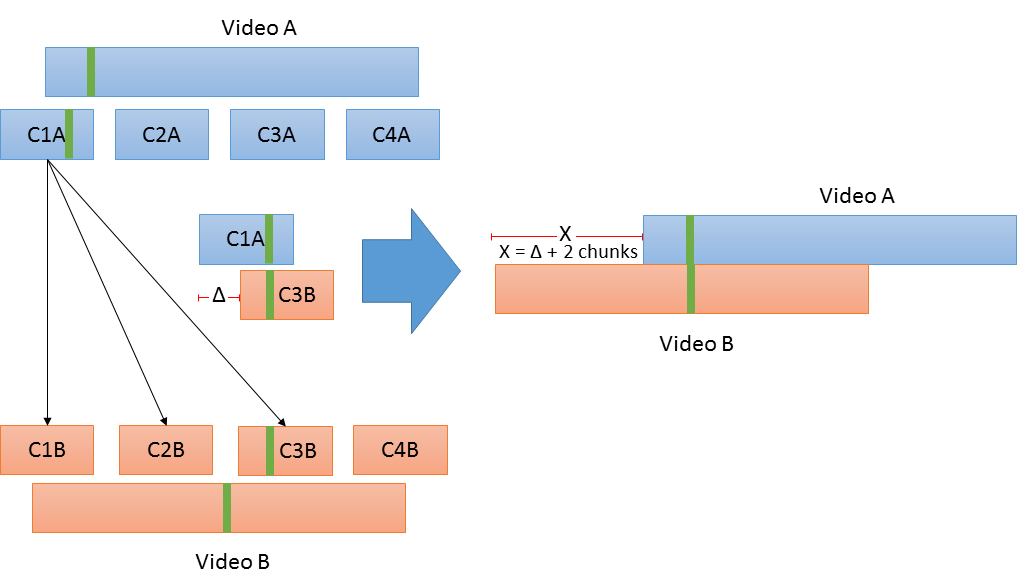
\includegraphics[scale=0.35] {figure/chunks}}
	\caption{Chunk Synchronization Method}
	\label{chunks_process}
\end{figure}

When two chunks associated with two videos are synchronized, all the contents of these two videos will also be synchronized. This happens because as described in the introduction, we consider the videos as continuous. And if comparing all chunks from both videos, we can't find any synchronization point, those two probably have no synchronization point. We say probably, because there is a possibility that the crowd fails in its tasks. To reduce this possibility, there are measures that can be taken such as assessing the crowd for better contributions. We however do not discuss this issue in this paper, as our scope focus on the synchronization process only. Another important consideration here is that this approach can fall in the worst case when there is no synchronization point, and all chunks will be compared, and will fail. On the other hand, if there is an synchronization point, we can find it in the first comparison.